\documentclass[10pt,english,aspectratio=169]{beamer}

\usetheme{default}

\usepackage{xstring}
\usepackage{pgfpages}
%\makeatletter
%\IfSubStr{\@classoptionslist}{handout}
%  {\pgfpagesuselayout{2 on 1}[letterpaper,border shrink=5mm]}
%  {}
%\makeatother

\usepackage{amsmath,amssymb,amsthm}
\usepackage{stmaryrd}
\usepackage{enumerate}
\usepackage{stfloats}
\usepackage{bbm}
\usepackage{pdfpages}
\usepackage{framed}

\usepackage[most]{tcolorbox}
\tcbset{highlight math style={enhanced,
  colframe=white,colback=yellow!15,arc=8pt,boxrule=1pt,
  }}
  
\usepackage{tikz,pgf,pgfplots}
\usepackage{algorithm,algorithmic}
\usepgflibrary{shapes}
\usetikzlibrary{%
  arrows,%
  arrows.meta,
  backgrounds,
  shapes.misc,% wg. rounded rectangle
  shapes.arrows,%
  shapes,%
  calc,%
  chains,%
  matrix,%
  positioning,% wg. " of "
  scopes,%
  decorations.pathmorphing,% /pgf/decoration/random steps | erste Graphik
  shadows,%
  backgrounds,%
  fit,%
  petri,%
  quotes
}

\tikzset{background rectangle/.style={
    fill=white,
  },
  use background/.style={    
    show background rectangle
  }
}

\setbeamersize{text margin left=10mm,text margin right=35mm}

\pgfplotsset{compat=1.12}

%\usetheme{Frankfurt}
%\usecolortheme{ldpc}
\useinnertheme{rounded}
\usecolortheme{whale}
\usecolortheme{orchid}

\newcommand{\ul}[1]{\underline{#1}}
\renewcommand{\Pr}{\mathbb{P}}

%% Setup slides and notes
\makeatletter
\IfSubStr{\@classoptionslist}{handout}
  {\def\slidesonly{}}{\def\slidesnotes{}}
\makeatother

%\setbeameroption{show notes on second screen=right} % Both
\ifdefined\notesonly
  \setbeameroption{show only notes} % Only notes
\fi
\ifdefined\slidesnotes
  \setbeameroption{show notes on second screen=right} % Both
\fi
\ifdefined\slidesonly
  \setbeameroption{hide notes} % Only slides
\fi
%\setbeamertemplate{note page}{\pagecolor{yellow!5}\vfill\insertnote\vfill}

\newcommand{\getpdfpages}[2]{\begingroup
  \setbeamercolor{background canvas}{bg=}
  \addtocounter{framenumber}{1}
  \includepdf[pages={#1},%
  pagecommand={%
    \expandafter\def\expandafter\insertshorttitle\expandafter{%
      \insertshorttitle\hfill\insertframenumber\,/\,\inserttotalframenumber}}%
  ]{#2}
  \endgroup}

\newcommand{\backupbegin}{
   \newcounter{finalframe}
   \setcounter{finalframe}{\value{framenumber}}
}
\newcommand{\backupend}{
   \setcounter{framenumber}{\value{finalframe}}
}

 \setbeamercolor{bibliography entry author}{fg=black}
 \setbeamercolor{bibliography entry title}{fg=black}
 \setbeamercolor{bibliography entry location}{fg=black}
 \setbeamercolor{bibliography entry note}{fg=black}
 
 \setbeamerfont{bibliography item}{size=\footnotesize}
 \setbeamerfont{bibliography entry author}{size=\footnotesize}
 \setbeamerfont{bibliography entry title}{size=\footnotesize}
 \setbeamerfont{bibliography entry location}{size=\footnotesize}
 \setbeamerfont{bibliography entry note}{size=\footnotesize}
 \setbeamertemplate{bibliography item}{\insertbiblabel}
 
\newlength\tikzwidth
\newlength\tikzheight


\newcommand{\mc}[1]{\mathcal{#1}}
\newcommand{\mbb}[1]{\mathbb{#1}}
%\newcommand{\expt}{\mbb{E}}
%\newcommand{\dd}{\mathrm{d}}
\newcommand{\Interior}[1]{\ensuremath{{#1}^{\circ}}}
\newcommand{\Closure}[1]{\ensuremath{\overline{#1}}}
\newcommand{\Complement}[1]{\ensuremath{{#1}^{c}}}

\newcommand{\Expect}{\ensuremath{\mathrm{E}}}
\newcommand{\vecnot}{\underline}
\newcommand{\RealNumbers}{\ensuremath{\mathbb{R}}}
\newcommand{\RationalNumbers}{\mathbb{Q}}
\newcommand{\ComplexNumbers}{\mathbb{C}}
\newcommand{\Real}{\mathrm{Re}}
\newcommand{\Span}{\mathrm{span}}
\newcommand{\Rank}{\mathrm{rank}}
\newcommand{\Nullity}{\mathrm{nullity}}
\newcommand{\Trace}{\mathrm{tr}}
\newcommand{\Diag}{\mathrm{diag}}
\newcommand{\dd}{\mathrm{d}}
\DeclareMathOperator*{\esssup}{ess\,sup}

% Use < , > inner product
\newcommand{\inner}[2]{{\left\langle #1 \mskip2mu , #2 \right\rangle}}
\newcommand{\tinner}[2]{{\langle #1 \mskip1mu , #2 \rangle}}

% Use < | > inner product
%\newcommand{\inner}[2]{{\left\langle #1 \mskip2mu \middle| \mskip2mu #2 \right\rangle}}
%\newcommand{\tinner}[2]{{\langle #1 \mskip1mu | \mskip1mu  #2 \rangle}}




\def\checkmark{\tikz\fill[scale=0.4](0,.35) -- (.25,0) -- (1,.7) -- (.25,.15) -- cycle;}
\def\greencheck{{\color{green}\checkmark}}
\def\scalecheck{\resizebox{\widthof{\checkmark}*\ratio{\widthof{x}}{\widthof{\normalsize x}}}{!}{\checkmark}}
\def\xmark{\tikz [x=1.4ex,y=1.4ex,line width=.2ex, red] \draw (0,0) -- (1,1) (0,1) -- (1,0);}
\def\redx{{\color{red}\xmark}}

\renewcommand{\footnotesep}{-2pt}


\begin{document}



\title{ECE 586: Vector Space Methods \\ Lecture 6 Flip Video: Complete Metric Spaces}
\author{Henry D. Pfister \\ Duke University}
\date{}
%\date{August 20th, 2020}
%\maketitle

\setbeamertemplate{navigation symbols}{}

\begin{frame}[plain]
	\titlepage
	
	\note{
		\vspace{8mm}
		\begin{enumerate}
			\setlength\itemsep{3mm}
			\color{red}
			\item Welcome to the sixth video lecture for ECE 586, Vector Space Methods. \\[2mm]
			Today, we'll discuss complete metric spaces and the contraction mapping theorem.
		\end{enumerate}
	}
\end{frame}

\addtocounter{framenumber}{-1}
\setbeamertemplate{navigation symbols}{\textcolor{blue}{\footnotesize \insertframenumber ~/ \inserttotalframenumber}}



\begin{frame}<1-3> \frametitle{2.1.3: Completeness}

\begin{definition}<1->
A metric space $(X,d)$ is said to be \textcolor{blue}{complete} if every Cauchy sequence in $(X,d)$ converges to a limit $x \in X$.
\end{definition}

\begin{example}<2->
Consider the sequence $x_n \in \mathbb{Q}$ defined by $x_1 = 2$ and $\smash{x_{n+1} = \frac{1}{2}x_n + 1/x_n}$.
For this sequence, one can show that $|x_n - \sqrt{2}|\to 0$. Since $\sqrt{2}$ is not rational, however, this shows the standard \textcolor{red}{metric space of rationals is not complete}.
\end{example}

\begin{alertblock}{Key Point}<3->
The standard metric space of real numbers is a complete metric space.
This can be proven by starting with Zermelo-Fraenkel (ZF) set theory and associating the real numbers with Cauchy sequences of rational numbers.  The proof of this is not covered in this class but is available on the website.
\end{alertblock}

\note{
	\vspace{2mm}
	\begin{enumerate}[<alert@+>]
		\footnotesize
		\setlength\itemsep{3mm}
		\item Read.  Completeness is very useful property for analysis and, thus, researchers prefer to setup problems in complete spaces if possible.
		\item Read.
		\item I should note that (read)
	\end{enumerate}
}

\end{frame}


\begin{frame}<1-4> \frametitle{2.1.3: Dense Subsets}

\begin{definition}<1->
A subset $A$ of a metric space $(X,d)$ is \textcolor{blue}{dense} in $X$ if every $x\in X$ is a limit point of the set $A$.
This is equivalent to the closure $\overline{A}$ being equal to $X$.
\end{definition}

\begin{example}<2->
The rational numbers are a dense subset of the real numbers because every real number is the limit of a sequence of rational numbers.
\end{example}

\begin{definition}<3->
The \textcolor{blue}{completion} of a metric space $(X,d_X)$ consists of a complete metric space $(Y,d_Y)$ and an isometry $\phi  \colon X \rightarrow Y$ such that $\phi(X)$ is a dense subset of $Y$.
Moreover, the completion is unique up to isometry.
\end{definition}

\begin{alertblock}{Remark}<4->
One can always complete a metric space $(X,d)$ by considering Cauchy sequences of elements in $X$.
\end{alertblock}

\note{
	\vspace{2mm}
	\begin{enumerate}[<alert@+>]
		\footnotesize
		\setlength\itemsep{3mm}
		\item Read.  
		\item Read.  Later, we will see that having a countably dense subset can be useful when proving things.
		\item Read.  For example, think of $X$ as the rational numbers, $Y$ as the real numbers, and $\phi$ as he mapping that embeds the rational numbers io the real numbers.  I should also note that an isometry is a function between metric spaces that preserves pairise distances.
		\item For example, if a metric space is not complete, then some of its natural limit points have been left out.  This can be repaired by creating new points associated with Cauchy sequences that don't converge.
	\end{enumerate}
}

\end{frame}


\begin{frame}<1-3> \frametitle{2.1.3: A Space of Continuous Functions}

\begin{example}
Let $X=C[-1,1]$ be the space of continuous functions that map $[-1,1]$ to $\mathbb{R}$ and satisfy $\left\| f \right\|_2 < \infty$, where $\left\| f \right\|_2$ denotes the $L^2$ norm \vspace{-3mm}
\begin{equation*}
\left\| f \right\|_2 \triangleq \left( \int_{-1}^1 |f(t)|^2 dt \right)^{1/2} \vspace{-2mm}
\end{equation*}
This set forms a metric space $(X,d)$ when equipped with the distance \vspace{-3mm}
\[ d(f, g) \triangleq \left\| f - g \right\|_2
= \left( \int_{-1}^1 |f(t) - g(t)|^2 dt \right)^{1/2} \vspace{-2mm} \]
Now, consider the sequence of functions $f_n(t)$ given by \vspace{-2mm}
\begin{equation*}
f_n(t) \triangleq \left\{ \begin{array}{ll}
0 & t \in \left[ -1, -\frac{1}{n} \right] \\
\frac{nt}{2} + \frac{1}{2} & t \in \left( -\frac{1}{n}, \frac{1}{n} \right) \\
1 & t \in \left[ \frac{1}{n}, 1 \right] 
\end{array} \right\} \vspace{-1mm}
\end{equation*}

\uncover<3->{One can show that \textcolor{red}{this is a Cauchy sequence in $(X,d)$} \\
But, \textcolor{red}{it does not converge} to a continuous function in $C[-1,1]$}
\end{example}

\uncover<2->{%
\begin{tikzpicture}[overlay,remember picture,shift={(10.75,1.5)}]
\draw[fill=brown!30,rounded corners] (-1.3,-0.9) rectangle (4.1,3.15);
\begin{axis}[
    %title={Continuous Functions},
    axis background/.style={fill=white},
	small,
	font=\small,
    width=53mm,
    xlabel={$t$},
    xlabel near ticks,
    xmin=-1, xmax=1,
    xmajorgrids,
    ylabel={$f_n(t)$},
    ylabel near ticks,
    ymajorgrids,
    legend style={font=\tiny},
    legend pos=north west]

\addplot[darkgray,line width=1pt] coordinates {
    (-1,0) (-0.5,0) (0.5,1) (1,1)};
\addlegendentry{$n = 2$}

\addplot[blue,line width=1pt] coordinates {
    (-1,0) (-0.25,0) (0.25,1) (1,1)};
\addlegendentry{$n = 4$}

\addplot[magenta,line width=1pt] coordinates {
    (-1,0) (-0.125,0) (0.125,1) (1,1)};
\addlegendentry{$n = 8$}
\end{axis}
\end{tikzpicture}
}

\note{
	\vspace{2mm}
	\begin{enumerate}[<alert@+>]
		\footnotesize
		\setlength\itemsep{3mm}
		\item Read.
		\item This figure shows the first few functions in the sequence and we see it's a sequence of continuous functions converging to the step function.  The key problem is that the limit function is not continuous and therefore not in the set $X$.
		\item Analytically, (read).
	\end{enumerate}
}

\end{frame}




\begin{frame}<1-2> \frametitle{2.1.3: Contractions on Metric Spaces}

\begin{definition}<1->
Let $A$ be a subset of a metric space $(X,d)$ and $f \colon X \rightarrow X$ be a function.
Then, $f$ is a \textcolor{blue}{contraction} on $A$ if $f(A) \subseteq A$ and there exists a constant $\gamma < 1$ such that $d \left( f(x),f(y) \right) \leq \gamma  d(x,y)$ for all $x,y\in A$.
\end{definition}

\begin{example}<2->
\begin{minipage}{0.52\textwidth}
Consider the metric space $X=[0,1]$ with absolute distance.
Define $f\colon X \to X$ with $f(x) = 1-\frac{1}{2}x$ and observe that \vspace{-2mm} \[d\big(f(x),f(y)\big)=|f(x)-f(y)| = \frac{1}{2}|x-y| \] \\[-2mm]
\end{minipage}
\hfill
\begin{minipage}{0.43\textwidth}
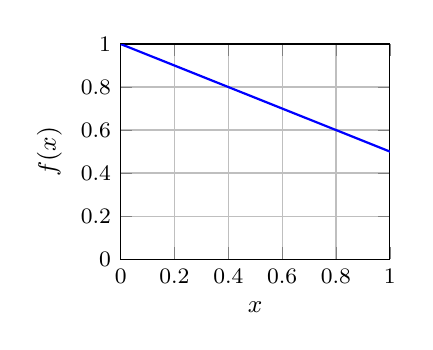
\begin{tikzpicture}%[overlay,remember picture,shift={(12.5,-0.5)}]
\begin{axis}[
	small,
	font=\small,
    width=50mm,
    xlabel={$x$},
    xlabel near ticks,
    xmin=0, xmax=1,
    xmajorgrids,
    ylabel={$f(x)$},
    ylabel near ticks,
    ymin=0,
    ymax=1,
    ymajorgrids,
    legend style={font=\tiny},
    legend pos=north west]

    \addplot[blue,thick] { 1 - x/2 };
\end{axis}
\end{tikzpicture}
\end{minipage}
\end{example}

\note{
	\vspace{2mm}
	\begin{enumerate}[<alert@+>]
		\footnotesize
		\setlength\itemsep{3mm}
		\item Read.
		\item Read. Thus, $f$ is a contraction on $X$ with contraction coefficient $\frac{1}{2}$.  The figure shows the graph of $f$.
	\end{enumerate}
}

\end{frame}


\begin{frame}{2.1.3: Contraction Mapping Theorem}

\begin{theorem}[Contraction Mapping Theorem]<1->
Let $(X,d)$ be a complete metric space and $f$ be contraction on a closed subset $A \subseteq X$.
Then, 
\begin{itemize}
\setlength\itemsep{3mm}
  \item $f$ has a unique fixed point $x^* \in A$ such that $f(x^*) = x^*$ and the sequence $x_{n+1} = f(x_n)$ converges to $x^*$ from any initial $x_1 \in A$
  \item Also, $x_n$ satisfies the error bounds (for contraction coefficient $\gamma$): \vspace{-2mm} \begin{align*} d(x^*,x_n) &\leq \gamma^{n-1} d(x^*,x_1) \\ d(x^*,x_{n+1}) &\leq d(x_n,x_{n+1})\gamma /(1-\gamma) \end{align*}
\end{itemize}
\end{theorem}

\note{
	\vspace{2mm}
	\begin{enumerate}[<alert@+>]
		\footnotesize
		\setlength\itemsep{3mm}
		\color{red}
		\item First, we look at the figure.  It illustrates a function $f$ that is a contraction on the closed subset $A$ (which is outlined in blue). Because of this, the image of $A$ under $f$ (which is outlined in purple) lies inside of $A$.  Likewise, the image of the set $f(A)$ under $f$ (which is outlined in red) lies inside the set $f(A)$.  \\ [2mm] Now, look at the theorem. Read \\ [2mm] If this process were continued, the image of $A$ under the $n$-fold composition of $f$ ith itself would shrink to the fixed point $x^*$.  
	\end{enumerate}
}

  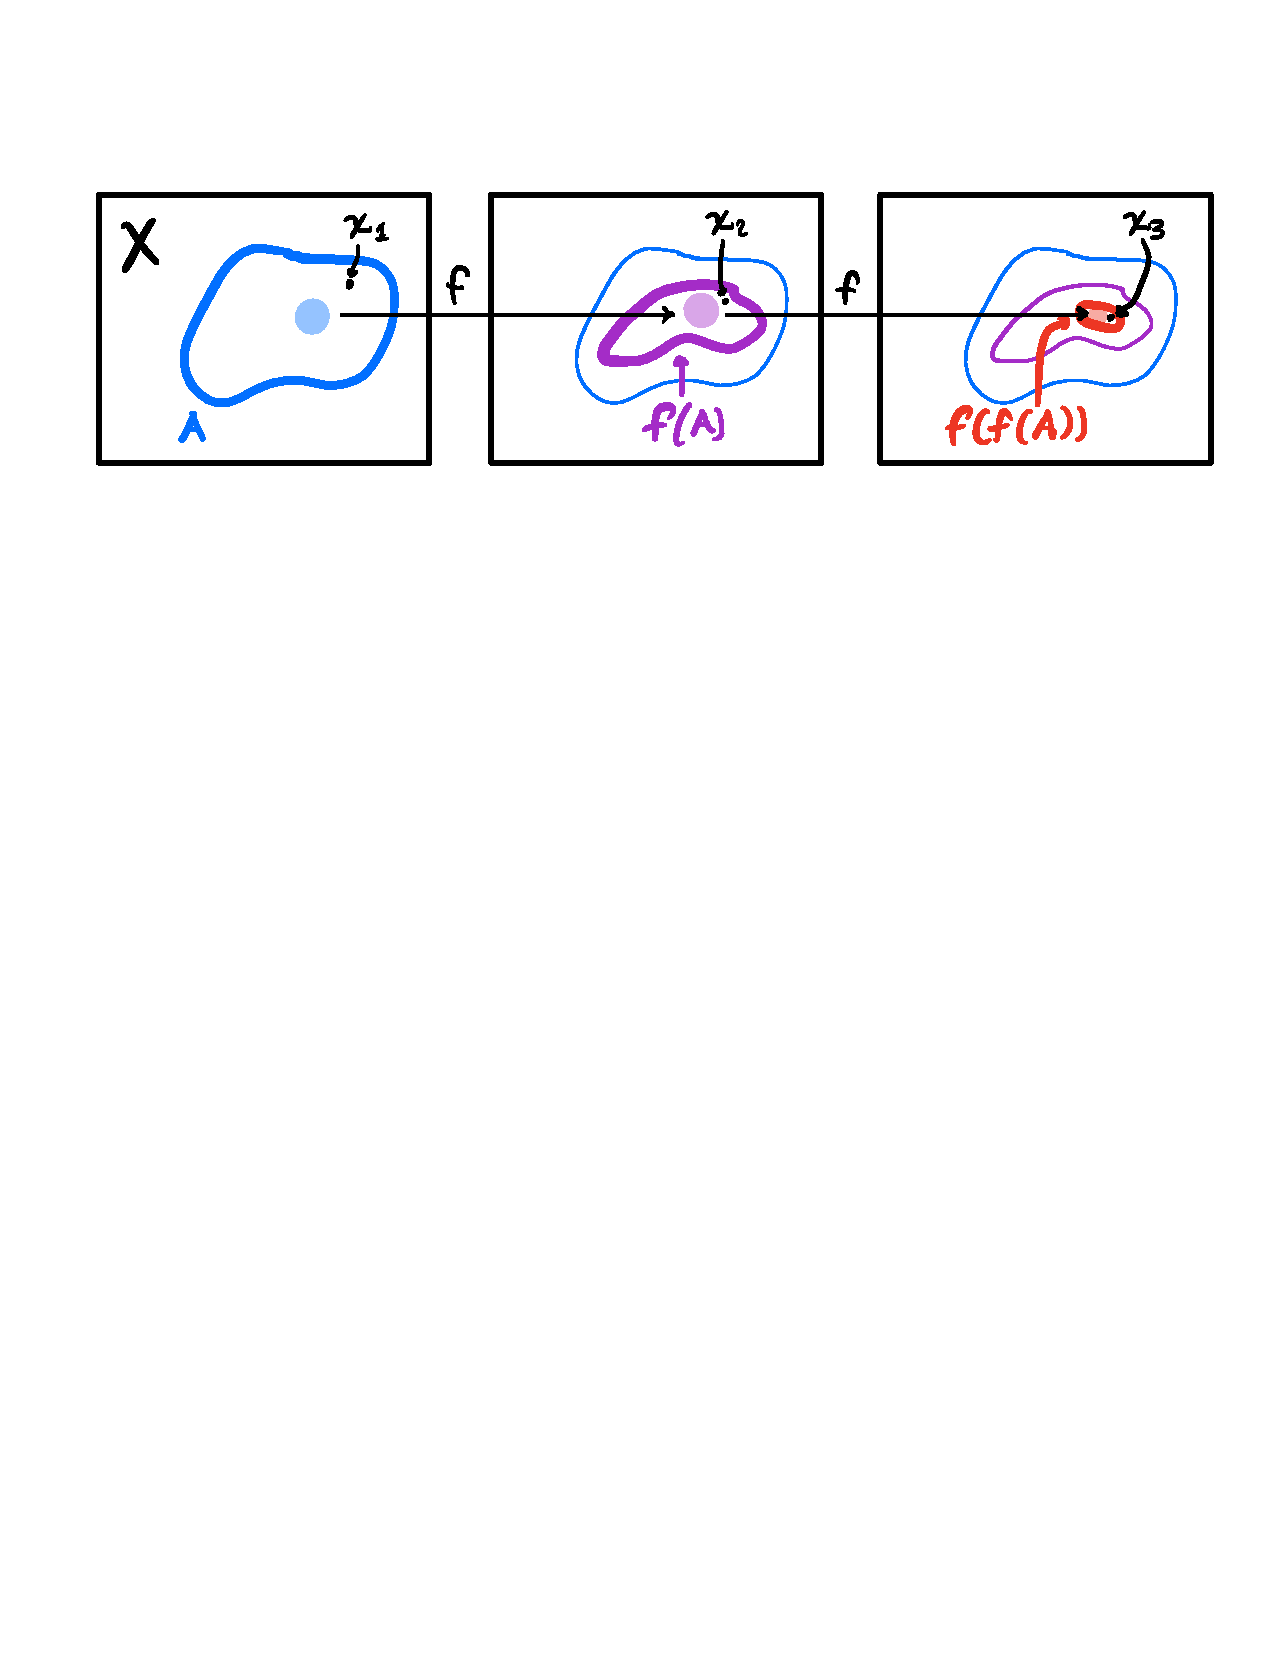
\includegraphics[width=\textwidth]{figures/ch2_contraction_mapping}

\end{frame}

\begin{frame}<1-3> \frametitle{2.1.3: Applications of the Contraction Mapping Theorem}

Several important results in applied mathematics have relatively simple proofs based on the contraction mapping theorem:
\vspace{1mm}

\begin{itemize}
\setlength\itemsep{3mm}
\item<1-> \textcolor{blue}{Picard's uniqueness theorem for differential equations} \vspace{1mm}
\begin{itemize} 
  \setlength\itemsep{1.5mm}
  \item Differential equation $y'(t) = f(t,y(t))$ for $t\in [a,b]$ with $y(a)=y_0$ 
  \item  Assume $f(t,y)$ is Lipschitz continuous in $y$ for $t\in [a,b]$
  \item Then, the solution $y(t)$ exists and is unique for $t\in [a,b]$
\end{itemize}
\item<2-> \textcolor{blue}{Implicit function theorem} \vspace{1mm}
\begin{itemize} 
  \setlength\itemsep{1.5mm}
  \item Let $f\colon \mathbb{R}^n \times \mathbb{R}^{m} \to \mathbb{R}^m$ be continuously differentiable on an open set $A$
  \item Let $g\colon \mathbb{R}^n \to \mathbb{R}^{m}$ be defined implicitly by $f(x,g(x))=0$
  \item For $x_0\in A$, assume $f(x_0,y_0)=0$ and $y$-Jacobian invertible at $(x_0,y_0)$
  \item Then, $g(x)$ exists and is unique in some neighborhood of $x_0$
\end{itemize}
\item<3-> \textcolor{blue}{Dynamic Programming for a Markov Decision Process (MDP)} \vspace{1mm}
\begin{itemize} 
  \setlength\itemsep{1.5mm}
  \item State-action $(s,a)$ defines probability $p(s'|s,a)$ and reward $R(s,a)$
  \item Finite state + discounted reward $\Rightarrow$ unique stationary optimal policy
\end{itemize}
\end{itemize}

\note{
	\vspace{2mm}
	\begin{enumerate}[<alert@+>]
		\footnotesize
		\setlength\itemsep{3mm}
		\item Read.  There is an optional homework problem that outlines this proof for a special case of this theorem.  
		\item Read.  which provides a method prove the local uniqueness of a function that is defined implicitly.
		\item Read.  This is related to reinforcement learning and other methods by which computers can learn to play video games.
	\end{enumerate}
}

\end{frame}

\begin{frame}<1-6> \frametitle{2.1.3: Concrete Example of the Contraction Mapping Theorem}

\vspace{1mm}
\begin{minipage}{0.45\textwidth}
Starting from $x_1 = 0.2$, define the sequence $x_{n+1}= \cos(x_n)$ and plot the x-y pairs $(x_n,x_{n+1})$.  Each point is connected to the ``$y\!=\!x$'' line to emphasize the sequential path.
\end{minipage}
\begin{minipage}{0.5\textwidth}
\scalebox{0.72}{% This file was created by matlab2tikz v0.3.0.
% Copyright (c) 2008--2012, Nico Schlömer <nico.schloemer@gmail.com>
% All rights reserved.
% 
% The latest updates can be retrieved from
%   http://www.mathworks.com/matlabcentral/fileexchange/22022-matlab2tikz
% where you can also make suggestions and rate matlab2tikz.
% 
% 
% 
% defining custom colors
\definecolor{mycolor1}{rgb}{0,0.447,0.741}
\definecolor{mycolor2}{rgb}{0.85,0.325,0.098}
\definecolor{mycolor3}{rgb}{1,0,1}
\begin{tikzpicture}
\begin{axis}[%
width=3in,
height=2.5in,
every outer x axis line/.append style={darkgray!60!black},
every x tick label/.append style={font=\color{darkgray!60!black}},
grid=major,
xmin=0, xmax=1,
xlabel={$x_n$},
every outer y axis line/.append style={darkgray!60!black},
every y tick label/.append style={font=\color{darkgray!60!black}},
ymin=0, ymax=1,
ylabel={$x_{n+1}$}]
\addplot [
thick,
color=mycolor1,
solid,
forget plot
]
coordinates{
 (0,0)(0.01,0.01)(0.02,0.02)(0.03,0.03)(0.04,0.04)(0.05,0.05)(0.06,0.06)(0.07,0.07)(0.08,0.08)(0.09,0.09)(0.1,0.1)(0.11,0.11)(0.12,0.12)(0.13,0.13)(0.14,0.14)(0.15,0.15)(0.16,0.16)(0.17,0.17)(0.18,0.18)(0.19,0.19)(0.2,0.2)(0.21,0.21)(0.22,0.22)(0.23,0.23)(0.24,0.24)(0.25,0.25)(0.26,0.26)(0.27,0.27)(0.28,0.28)(0.29,0.29)(0.3,0.3)(0.31,0.31)(0.32,0.32)(0.33,0.33)(0.34,0.34)(0.35,0.35)(0.36,0.36)(0.37,0.37)(0.38,0.38)(0.39,0.39)(0.4,0.4)(0.41,0.41)(0.42,0.42)(0.43,0.43)(0.44,0.44)(0.45,0.45)(0.46,0.46)(0.47,0.47)(0.48,0.48)(0.49,0.49)(0.5,0.5)(0.51,0.51)(0.52,0.52)(0.53,0.53)(0.54,0.54)(0.55,0.55)(0.56,0.56)(0.57,0.57)(0.58,0.58)(0.59,0.59)(0.6,0.6)(0.61,0.61)(0.62,0.62)(0.63,0.63)(0.64,0.64)(0.65,0.65)(0.66,0.66)(0.67,0.67)(0.68,0.68)(0.69,0.69)(0.7,0.7)(0.71,0.71)(0.72,0.72)(0.73,0.73)(0.74,0.74)(0.75,0.75)(0.76,0.76)(0.77,0.77)(0.78,0.78)(0.79,0.79)(0.8,0.8)(0.81,0.81)(0.82,0.82)(0.83,0.83)(0.84,0.84)(0.85,0.85)(0.86,0.86)(0.87,0.87)(0.88,0.88)(0.89,0.89)(0.9,0.9)(0.91,0.91)(0.92,0.92)(0.93,0.93)(0.94,0.94)(0.95,0.95)(0.96,0.96)(0.97,0.97)(0.98,0.98)(0.99,0.99)(1,1) 
};
\addplot [
very thick,
color=red, %mycolor2,
solid,
forget plot
]
coordinates{
 (0,1)(0.01,0.999950000416665)(0.02,0.999800006666578)(0.03,0.999550033748988)(0.04,0.999200106660978)(0.05,0.998750260394966)(0.06,0.998200539935204)(0.07,0.99755100025328)(0.08,0.996801706302619)(0.09,0.995952733011994)(0.1,0.995004165278026)(0.11,0.993956097956697)(0.12,0.992808635853866)(0.13,0.991561893714788)(0.14,0.990215996212637)(0.15,0.988771077936042)(0.16,0.987227283375627)(0.17,0.985584766909561)(0.18,0.983843692788121)(0.19,0.98200423511727)(0.2,0.980066577841242)(0.21,0.978030914724148)(0.22,0.975897449330606)(0.23,0.973666395005375)(0.24,0.97133797485203)(0.25,0.968912421710645)(0.26,0.966389978134513)(0.27,0.963770896365891)(0.28,0.961055438310771)(0.29,0.958243875512697)(0.3,0.955336489125606)(0.31,0.952333569885713)(0.32,0.949235418082441)(0.33,0.946042343528387)(0.34,0.942754665528346)(0.35,0.939372712847379)(0.36,0.935896823677935)(0.37,0.932327345606034)(0.38,0.92866463557651)(0.39,0.924909059857313)(0.4,0.921060994002885)(0.41,0.917120822816605)(0.42,0.913088940312308)(0.43,0.908965749674885)(0.44,0.904751663219963)(0.45,0.900447102352677)(0.46,0.896052497525525)(0.47,0.891568288195329)(0.48,0.886994922779284)(0.49,0.882332858610121)(0.5,0.877582561890373)(0.51,0.872744507645751)(0.52,0.86781917967765)(0.53,0.862807070514761)(0.54,0.857708681363824)(0.55,0.852524522059506)(0.56,0.847255111013416)(0.57,0.841900975162269)(0.58,0.836462649915187)(0.59,0.830940679100164)(0.6,0.825335614909678)(0.61,0.819648017845479)(0.62,0.813878456662534)(0.63,0.808027508312152)(0.64,0.802095757884293)(0.65,0.796083798549056)(0.66,0.789992231497365)(0.67,0.783821665880849)(0.68,0.777572718750928)(0.69,0.771246014997107)(0.7,0.764842187284488)(0.71,0.758361875990508)(0.72,0.751805729140895)(0.73,0.74517440234487)(0.74,0.738468558729588)(0.75,0.731688868873821)(0.76,0.724836010740905)(0.77,0.717910669610943)(0.78,0.710913538012277)(0.79,0.703845315652236)(0.8,0.696706709347165)(0.81,0.689498432951747)(0.82,0.682221207287613)(0.83,0.674875760071267)(0.84,0.667462825841308)(0.85,0.659983145884982)(0.86,0.652437468164052)(0.87,0.644826547240001)(0.88,0.63715114419858)(0.89,0.629412026573697)(0.9,0.621609968270664)(0.91,0.613745749488812)(0.92,0.605820156643463)(0.93,0.597833982287298)(0.94,0.589788025031098)(0.95,0.581683089463883)(0.96,0.573519986072457)(0.97,0.565299531160354)(0.98,0.557022546766217)(0.99,0.548689860581588)(1,0.54030230586814) 
};
\addplot [
thick,
color=mycolor3,
dashed,
forget plot
]
coordinates{
 (0.2,0.2)(0.2,0.980066577841242)(0.980066577841242,0.980066577841242) 
};
\addplot [
thick,
color=mycolor3,
dashed,
forget plot
]
coordinates{
 (0.980066577841242,0.980066577841242)(0.980066577841242,0.556967252809642)(0.556967252809642,0.556967252809642) 
};
\addplot [
thick,
color=mycolor3,
dashed,
forget plot
]
coordinates{
 (0.556967252809642,0.556967252809642)(0.556967252809642,0.848862165658271)(0.848862165658271,0.848862165658271) 
};
\addplot [
thick,
color=mycolor3,
dashed,
forget plot
]
coordinates{
 (0.848862165658271,0.848862165658271)(0.848862165658271,0.660837551116615)(0.660837551116615,0.660837551116615) 
};
\addplot [
thick,
color=mycolor3,
dashed,
forget plot
]
coordinates{
 (0.660837551116615,0.660837551116615)(0.660837551116615,0.789478437766868)(0.789478437766868,0.789478437766868) 
};
\addplot [
thick,
color=mycolor3,
dashed,
forget plot
]
coordinates{
 (0.789478437766868,0.789478437766868)(0.789478437766868,0.704215713341993)(0.704215713341993,0.704215713341993) 
};
\addplot [
thick,
color=mycolor3,
dashed,
forget plot
]
coordinates{
 (0.704215713341993,0.704215713341993)(0.704215713341993,0.762119561760661)(0.762119561760661,0.762119561760661) 
};
\addplot [
thick,
color=mycolor3,
dashed,
forget plot
]
coordinates{
 (0.762119561760661,0.762119561760661)(0.762119561760661,0.723374172105571)(0.723374172105571,0.723374172105571) 
};
\addplot [
thick,
color=mycolor3,
dashed,
forget plot
]
coordinates{
 (0.723374172105571,0.723374172105571)(0.723374172105571,0.749576576331493)(0.749576576331493,0.749576576331493) 
};
\end{axis}
\end{tikzpicture}%}
\end{minipage}
\vspace{0mm}

\begin{itemize}
\setlength\itemsep{1.25mm}
\item<1-> Let $X=[0,1]$ and define $f\colon X\to X$ via $f(x)=\cos(x)$

\item<2-> $\cos([0,1]) = [\cos(1),1]$ because $\cos(x)$ decreasing on $[0,\pi]$

\item<3-> Mean value theorem: $f(y)-f(x) = f'(t) (y-x)$ for some $t\in [x,y]$

\item<4-> $f'(t) = -\sin(t)$ and $\sin([0,1]) = [0,\sin(1)]$ with $\sin(1) \approx 0.84$

\item<5-> $| \cos(y) - \cos(x) \,| \leq 0.85 \, |y-x|$ $\;\Rightarrow$ \textcolor{blue}{$f(x)$ is a contraction on $[0,1]$}

\item<6-> $x_{n+1} \!= \cos(x_n)$  converges to \textcolor{blue}{unique fixed point $x^* \!= \cos(x^*) \!\approx\! 0.739$}
\end{itemize}

\note{
	\vspace{2mm}
	\begin{enumerate}[<alert@+>]
		\footnotesize
		\setlength\itemsep{3mm}
		\item Read.  $cos(x)$ is plotted in red and, for the definition to make sense, one first needs to check that $cos(x) \in [0,1]$ whenever $x\in [0,1]$.
		\item The red curve above proves this numerically. Analytically, we see that (read).
		\item To show that $cos(x)$ is a contraction, we use the (read).
		\item Next, we note that the derivative (read).
		\item This implies that (read)
		\item Thus, the contraction mapping theorem implies that the sequence
	\end{enumerate}
}

\end{frame}  

\begin{frame} \frametitle{Next Steps}

\begin{itemize}
\setlength\itemsep{5mm}
\item To continue studying after this video -- \vspace{2mm}

\begin{itemize}
 \setlength\itemsep{3mm}
 \item Try the suggested reading: Course Notes EF 2.1.3
 \item Or the optional reading: MMA 2.1
 \item Also, look at the problems in Assignment 3
\end{itemize}
\end{itemize}

\note{
	\vspace{8mm}
	\begin{enumerate}
		\setlength\itemsep{3mm}
		\color{red}
		\item Here are some options to continue learning this material. (read) \\ [2mm]  That's it for today.  So, I'll see you next time.
	\end{enumerate}
}

\end{frame}


\end{document}


\begin{frame}{2.1.4: Compactness}

\begin{definition}<1->
A metric space $(X,d)$ is \textcolor{blue}{totally bounded} if, for any $\epsilon > 0$, there exists a finite set of $B_d (x,\epsilon)$ balls that cover (i.e., whose union equals) $X$.
\end{definition}

\begin{definition}<2->
A metric space is \textcolor{blue}{compact} if it is complete~and~totally~bounded.
\end{definition}

\begin{itemize}
\setlength\itemsep{3mm}
\item<3-> Examples \vspace{1mm}
\begin{itemize} 
  \setlength\itemsep{1.5mm}
  \item The closed interval $[0,1]\subset \RealNumbers$ is compact
  \item A subset of Euclidean $\RealNumbers^n$ is compact iff it is closed and bounded
  \item But, the standard metric space of real numbers is not compact because it is not totally bounded.
\end{itemize}

\end{itemize}

\begin{theorem}<4>
A closed subset $A$ of a compact space $X$ is itself a compact space.
\end{theorem}

\end{frame}

\begin{frame}{2.1.4: Compactness and Sequences}

\begin{definition}<1->
Let $x_1,x_2,\ldots \in X$ be a sequence and $n_1,n_2,\ldots\in \mathbb{N}$ be
a strictly increasing sequence.
Then, $x_{n_1},x_{n_2},\ldots$ is called \textcolor{blue}{subsequence}.
\end{definition}

\begin{theorem}<2->
A sequence in a compact metric space has a subsequence that converges.
\end{theorem}

\begin{example}<3->
For the compact metric space $X=[-2,2]\subset \mathbb{R}$ with absolute distance, let $x_n = (-1)^n + \frac{1}{n}$.
Then, subsequence $x_2,x_4,x_6,\ldots$ converges to 1.
\end{example}

\begin{itemize}
\item<3-> Sketch proof on whiteboard in pictures
\end{itemize}

\end{frame}

\begin{frame}{2.1.4: Properties of Real Numbers}

\begin{itemize}
\setlength\itemsep{3mm}
\item<1-> Let us consider extreme values for sets of real numbers \vspace{1mm}

\begin{itemize} 
  \setlength\itemsep{1.5mm}
  \item Extended Real Numbers: $\overline{\RealNumbers} \triangleq \RealNumbers \cup \{ \infty,-\infty\}$
  \item Defines \textcolor{blue}{compact metric space} with metric $d_{\overline{\RealNumbers}} (x,y) \triangleq |\frac{x}{1+|x|} - \frac{y}{1+|y|}|$
  \item ``$x_n \to \infty$'' equivalent to ``$\forall M>0, \, \exists N\in \mathbb{N}, \, \forall n>N, \, x_n > M$''
\end{itemize}
\end{itemize}

\begin{definition}<2->
The \textcolor{blue}{supremum} (or least upper bound) of $X\subseteq \RealNumbers$, denoted \textcolor{blue}{$\sup X$}, is the smallest extended real number $M \in \overline{\RealNumbers}$ such that $x\leq M$ for all $x\in X$.
%It is always well-defined and equals $-\infty$ if $X=\emptyset$.
\end{definition}

\begin{lemma}[supremum sequence]<3->
Let $X$ be a metric space and $f \colon X\rightarrow \RealNumbers$ be a function from $X$ to the real numbers.
Let $M = \sup f(A)$ for some non-empty $A \subseteq X$.
Then, there exists a sequence $x_1,x_2,\ldots \in A$ such that $\lim_n f(x_n) = M$.
\end{lemma}

\begin{itemize}
\item<4-> Sketch proof on whiteboard
\end{itemize}
  
\end{frame}


\begin{frame}{2.1.4: More Properties of Real Numbers}

\begin{definition}<1->
The \textcolor{blue}{maximum} of $X\subseteq \RealNumbers$, denoted \textcolor{blue}{$\max X$}, is the largest value achieved by the set.
It equals the supremum if $\sup X \in X$ and is \textcolor{red}{undefined} otherwise.
\end{definition}

\begin{example}<2->
$X = [1,2) \subset \mathbb{R}$ has $\sup X = 2$ and $\max X$ undefined. \\[1mm]
For $f(x)=\frac{1}{2-x}$, $f(X) = [1,\infty)$ and $\sup f(X) = \infty$.
\end{example}

\begin{itemize}
\item<3-> \textcolor{blue}{infimum}: $\inf X = - \left(\sup \, -\!X\right)$, where $-\!X = \{x\in \mathbb{R}\,|-\!x\in X\}$
\item<3-> \textcolor{blue}{minimum}: $\min X = - \left(\max \, -\!X \right)$, if it exists
\item<3-> supremum and infimum always well-defined but may equal $\pm \infty$
\end{itemize}



\begin{theorem}<4->
Any bounded non-decreasing sequence of real numbers converges to its supremum.
\end{theorem}

\end{frame}  


\begin{frame}{2.1.5: Sequences of Functions}

Let $(X,d_X)$ and $(Y,d_Y)$ be metric spaces and
$f_n \colon X \to Y$ for $n\in \mathbb{N}$ be a sequence of functions mapping $X$ to $Y$.

\begin{definition}
The sequence $f_n$ \textcolor{blue}{converges pointwise} to $f\colon X \to Y$ if, for all $x \in X$, \vspace{-1.5mm}
\[ \lim_{n\to \infty} f_n (x) = f(x) \vspace*{-0.5mm} \]

\end{definition}

\begin{definition}
The sequence $f_n$ \textcolor{blue}{converges uniformly} to $f \colon X \to Y$ if \vspace{-1.5mm}
\[ \forall \epsilon > 0, \, \exists N\in \mathbb{N}, \, \forall n>N, \, \forall x\in X, \, d_Y \left( f_n(x),f(x) \right) < \epsilon. \vspace*{-0.5mm} \]
\end{definition}

\begin{theorem}
If each $f_n$ is continuous and $f_n$ converges uniformly to $f \colon X \to Y$, then $f$ is continuous.
\end{theorem}

\end{frame}

\begin{frame}{2.1.5: Two Important Results}

\begin{theorem}
Let $X$ be a metric space and $f \colon X\rightarrow \RealNumbers$ be a continuous function from $X$ to $\mathbb{R}$.
If $A$ is a compact subset of $X$, then there exists $x\in A$ such that $f(x)=\sup f(A)$ (i.e., $f$ achieves a maximum on $A$).
\end{theorem}

\vspace{3mm}

\begin{theorem}
Let $(X,d)$ be a compact metric space and $C(X)$ be the set of continuous functions mapping $X$ to $\mathbb{R}$.
This set of functions, with the metric \vspace{-1.5mm} \[d_\infty (f,g) \triangleq \sup_{x\in X} |f(x)-g(x)| = \max_{x\in X} |f(x)-g(x)|, \vspace*{-1.5mm}\] defines a complete metric space.
\end{theorem}

Note: For $f,g\in C(X)$, $d_\infty$ metrizes uniform convergence because \vspace{-1.5mm} \[ \text{``}\max_{x\in X} |f(x)-g(x)| < \epsilon \text{''} \Leftrightarrow \text{``} \forall x\in X, |f(x) - g(x)| < \epsilon \text{''}. \]

\end{frame}


  
\backupbegin

%\begin{frame}
%\frametitle{Backup Slides}
%\begin{itemize}
%\item Slide numbers not included in denominator!
%\end{itemize}
%\end{frame}

%\begin{frame}[allowframebreaks]
%\frametitle{References}
%\bibliographystyle{alpha}
%\footnotesize
%\bibliography{IEEEabrv,WCLabrv,WCLbib,WCLnewbib}
%\end{frame}

\backupend

\end{document}
